% nnFoundation reading notes — compile with: latexmk -lualatex slides.tex
\documentclass[aspectratio=169,11pt]{beamer}

\usepackage{fontspec}
\usepackage{booktabs}
\usepackage{array}
\usepackage{colortbl}
\usepackage{pgfplots}
\pgfplotsset{compat=1.18}
\usetikzlibrary{arrows.meta}

% ---------- type ----------
\defaultfontfeatures{Path=/home/localssk23/.local/share/fonts/mdread/, Renderer=Node}
\setsansfont{Inter.ttf}[RawFeature={+tnum;axis={wght=400}}]
\newfontfamily\interbold{Inter.ttf}[RawFeature={+tnum;axis={wght=660}}]
\newfontfamily\titlefont{Literata.ttf}[RawFeature={axis={wght=470,opsz=48}}]
\newfontfamily\coverfont{Literata.ttf}[RawFeature={axis={wght=440,opsz=72}}]

% ---------- colour: architecture = hue, initialisation = tint ----------
\definecolor{paper}{HTML}{F4F6F7}   % light-box white
\definecolor{ink}{HTML}{1D2833}     % slate
\definecolor{rule}{HTML}{C5CED5}
\definecolor{cnn}{HTML}{2E5AA7}     % CNN: cobalt
\definecolor{vit}{HTML}{D99A12}     % ViT: PET-scale amber
\definecolor{unet}{HTML}{8C969F}    % nnU-Net: film grey
\colorlet{cnnS}{cnn!38!paper}       % from scratch = tint
\colorlet{vitS}{vit!38!paper}
\colorlet{other}{ink!40!paper}      % other foundation models

\setbeamercolor{background canvas}{bg=paper}
\setbeamercolor{normal text}{fg=ink}
\setbeamercolor{frametitle}{fg=ink}
\setbeamertemplate{navigation symbols}{}
\setbeamertemplate{frametitle}{%
  \vskip22pt\hskip6pt{\titlefont\fontsize{22}{26}\selectfont\insertframetitle}\vskip4pt}
\setlength{\leftmargini}{0pt}
\setbeamersize{text margin left=34pt, text margin right=34pt}

\newcommand{\sw}[1]{\textcolor{#1}{\rule{7pt}{7pt}}\hskip6pt}   % colour swatch
\newcommand{\best}[1]{{\interbold #1}}
\newcommand{\drow}[4]{% y, hollow value, filled value, colour
  \draw[#4, line width=2.2pt] (axis cs:#2,#1) -- (axis cs:#3,#1);
  \filldraw[fill=paper, draw=#4, line width=1.3pt] (axis cs:#2,#1) circle[radius=3.3pt];
  \fill[#4] (axis cs:#3,#1) circle[radius=3.8pt];}
\newcommand{\row}[4]{% y, arithmetic, geometric, colour
  \draw[#4, line width=2.4pt] (axis cs:#3,#1) -- (axis cs:#2,#1);
  \fill[#4] (axis cs:#2,#1) circle[radius=4.2pt];
  \filldraw[fill=paper, draw=#4, line width=1.4pt] (axis cs:#3,#1) circle[radius=3.6pt];
  \node[anchor=west, font=\small, text=ink, xshift=6pt] at (axis cs:#2,#1) {#2};}
\renewcommand{\arraystretch}{1.28}
\setlength{\aboverulesep}{0pt}\setlength{\belowrulesep}{0pt}
\arrayrulecolor{rule}

\pgfplotsset{
  deck/.style={
    axis line style={draw=none}, tick style={draw=none},
    ticklabel style={font=\small, text=ink},
    label style={font=\small, text=ink!75},
    grid style={draw=rule, line width=.4pt},
    legend style={draw=none, fill=none, font=\small, text=ink},
  }}

\begin{document}

% ------------------------------------------------------------------
{\setbeamertemplate{frametitle}{}
\begin{frame}
  \vfill
  \hskip6pt{\coverfont\fontsize{40}{46}\selectfont nnFoundation\par}
  \vskip10pt
  \hskip6pt{\titlefont\fontsize{20}{24}\selectfont\color{ink!70}3D foundation models for radiology\par}
  \vskip26pt
  \hskip6pt\textcolor{cnn}{\rule{70pt}{5pt}}\textcolor{vit}{\rule{70pt}{5pt}}
  \vskip30pt
  {\small\color{ink!75}
  \hskip6pt\begin{tabular}{@{}l l@{}}
  Original paper & \href{https://arxiv.org/abs/2609.26924}{arxiv.org/abs/2609.26924} \\
  Authors & DKFZ group, primarily \\
  Presented by & Lorena, Soumya \\
  Date & 24 September 2026 \\
  \end{tabular}}
  \vfill
\end{frame}}

% ------------------------------------------------------------------
\begin{frame}{Default, from scratch, pretrained}
\vskip14pt
{\small
\begin{tabular}{@{}l l l@{}}
\toprule
 & Network & Starting weights \\
\midrule
\sw{unet}nnU-Net Default & standard nnU-Net U-Net & random \\
\sw{cnnS}From scratch & ResEnc-L or Primus & random \\
\sw{cnn}Pretrained & ResEnc-L or Primus & MAE-pretrained encoder \\
 & & (2.1M unlabeled scans) \\
\midrule
All three & \multicolumn{2}{l}{then trained on the same labeled data} \\
\bottomrule
\end{tabular}}
\end{frame}

% ------------------------------------------------------------------
\begin{frame}{Two models, one recipe}
\vskip14pt
\begin{tabular}{@{}l l r l r@{}}
\toprule
Model & Backbone & Params & Pretraining & A100 hours \\
\midrule
\sw{cnn}nnF-CNN & ResEnc-L & 102M & MAE, 75\% masked & 500 \\
\sw{vit}nnF-ViT & Primus & 674M & MAE, 80\% masked & 12{,}500 \\
\bottomrule
\end{tabular}
\vskip24pt
\begin{tabular}{@{}l r@{}}
\toprule
Shared setup &  \\
\midrule
Pretraining loss & MSE, masked voxels \\
Input patch & 192$^3$ \\
Training steps & 625{,}000 \\
Batch size & 8 (CNN), 96 (ViT) \\
\bottomrule
\end{tabular}
\end{frame}

% ------------------------------------------------------------------
\begin{frame}{Compute}
\vskip4pt
\begin{tikzpicture}
\begin{axis}[deck,
  scale only axis, width=.52\textwidth, height=.30\textheight,
  xbar, bar width=9pt, bar shift=0pt, clip=false,
  xmin=0, xmax=60000, xtick={0,20000,40000,60000},
  xticklabels={0, 20k, 40k, 60k}, scaled x ticks=false,
  xmajorgrids, xlabel={A100 GPU-hours},
  ymin=-.6, ymax=3.6, ytick={0,...,3}, y dir=reverse,
  yticklabels={CNN pretraining, ViT pretraining, Method development, Downstream evaluation},
]
\addplot[fill=cnn, draw=none] coordinates {(500,0)};
\addplot[fill=vit, draw=none] coordinates {(12500,1)};
\addplot[fill=unet, draw=none] coordinates {(25000,2) (50000,3)};
\node[anchor=west, font=\small, text=ink, xshift=3pt] at (axis cs:500,0) {500};
\node[anchor=west, font=\small, text=ink, xshift=3pt] at (axis cs:12500,1) {12{,}500};
\node[anchor=west, font=\small, text=ink, xshift=3pt] at (axis cs:25000,2) {25{,}000};
\node[anchor=west, font=\small, text=ink, xshift=3pt] at (axis cs:50000,3) {50{,}000+};
\end{axis}
\end{tikzpicture}
\vskip10pt
{\small
\begin{tabular}{@{}l l @{\hskip28pt} l l@{}}
\toprule
GPU & NVIDIA A100 & Clusters & HoreKa, JUWELS \\
ViT pretraining run & 96 GPUs $\times$ 130 h & Fine-tuning GPU & 1 A100 40GB \\
Budget per SSL method & 400 h & Fine-tuning batch & 2 \\
\bottomrule
\end{tabular}}
\end{frame}

% ------------------------------------------------------------------
\begin{frame}{Pretraining data vs evaluation}
\vskip14pt
\small
\begin{columns}[T,onlytextwidth]
\column{.50\textwidth}
\begin{tabular}{@{}l r r@{}}
\toprule
Body region & Pretraining & Evaluation \\
\midrule
Brain & 290K & 29.3K \\
Head \& neck & 310K & 2.5K \\
Chest & 390K & 78.8K \\
Abdomen & 550K & 35.8K \\
Whole body / MSK & 370K & 13.1K \\
Unknown & 260K & -- \\
\midrule
\best{Total volumes} & \best{2.16M} & \best{160K} \\
\bottomrule
\end{tabular}
\column{.38\textwidth}
\begin{tabular}{@{}l r@{}}
\toprule
Pretraining source & Volumes \\
\midrule
Clinical partners & 1{,}315{,}227 \\
Research cohorts & 737{,}714 \\
Small public sets & 105{,}629 \\
\midrule
MRI & 71.7\% \\
CT & 26.6\% \\
PET & 1.7\% \\
\bottomrule
\end{tabular}
\end{columns}
\end{frame}

% ------------------------------------------------------------------
\begin{frame}{From 3.27M to 2.16M volumes}
\vskip2pt
\centering
\begin{tikzpicture}
\begin{axis}[deck,
  scale only axis, width=.56\textwidth, height=.56\textheight,
  xbar, bar width=8pt, bar shift=0pt, clip=false,
  xmin=0, xmax=500000, xtick={0,100000,...,500000},
  xticklabels={0,100k,200k,300k,400k,500k}, scaled x ticks=false,
  xmajorgrids, xlabel={Volumes removed},
  ymin=-.6, ymax=8.6, ytick={0,...,8}, y dir=reverse,
  yticklabels={Not CT / MRI / PET, NaN or Inf values, Segmentation masks, 4D series (diffusion{,} dynamic), Outliers after manual review, Overlap with downstream sets, Body-part regression failures, Fewer than 10 slices, Spacing above 8 mm},
]
\addplot[fill=unet, draw=none] coordinates {(180051,0) (67,1) (4192,2) (458754,3) (25456,4) (88477,5) (99716,6) (229693,7) (26478,8)};
\node[anchor=west, font=\small, text=ink, xshift=3pt] at (axis cs:180051,0) {180{,}051};
\node[anchor=west, font=\small, text=ink, xshift=3pt] at (axis cs:67,1) {67};
\node[anchor=west, font=\small, text=ink, xshift=3pt] at (axis cs:4192,2) {4{,}192};
\node[anchor=west, font=\small, text=ink, xshift=3pt] at (axis cs:458754,3) {458{,}754};
\node[anchor=west, font=\small, text=ink, xshift=3pt] at (axis cs:25456,4) {25{,}456};
\node[anchor=west, font=\small, text=ink, xshift=3pt] at (axis cs:88477,5) {88{,}477};
\node[anchor=west, font=\small, text=ink, xshift=3pt] at (axis cs:99716,6) {99{,}716};
\node[anchor=west, font=\small, text=ink, xshift=3pt] at (axis cs:229693,7) {229{,}693};
\node[anchor=west, font=\small, text=ink, xshift=3pt] at (axis cs:26478,8) {26{,}478};
\end{axis}
\end{tikzpicture}
\end{frame}

% ------------------------------------------------------------------
\begin{frame}{Pretraining scale vs prior models}
\vskip10pt
{\small
\begin{tabular}{@{}l l l r r@{}}
\toprule
Model & Input & Modality & 3D volumes (equivalent) & Eval datasets \\
\midrule
\sw{cnn}nnFoundation & 3D & CT, MRI, PET & \best{2{,}100{,}000} & \best{108} \\
CURIA & 2D & CT, MRI & 1{,}150{,}000\,$^\dagger$ & 23 \\
Prima & 3D & MRI & 221{,}147 & 10 \\
VoCo & 3D & CT & 160{,}000 & 48 \\
CT-FM & 3D & CT & 148{,}000 & 9 \\
MIS-FM & 3D & CT & 110{,}000 & 3 \\
Merlin & 3D & CT & 25{,}528 & 8 \\
VISTA3D & 3D & CT & 11{,}454 & 19 \\
SwinUNETR & 3D & CT, MRI & 5{,}050 & 11 \\
\bottomrule
\multicolumn{5}{@{}l}{\footnotesize\color{ink!60}$^\dagger$ 150K volumes + 200M 2D slices counted as slices $\div$ 200}
\end{tabular}}
\end{frame}

% ------------------------------------------------------------------
\begin{frame}{Picking the pretraining objective}
\vskip10pt
\begin{tabular}{@{}l r r r@{}}
\toprule
630K public volumes, 9 dev tasks & Seg Dice (5) & Cls AUROC (2) & Det mAP (2) \\
\midrule
\sw{cnn}CNN + MAE & \best{77.5} & 64.8 & \best{37.9} \\
\sw{cnn}CNN + contrastive & 76.0 & 70.8 & 34.6 \\
\sw{vit}ViT + MAE & 75.6 & \best{73.2} & 36.7 \\
\sw{vit}ViT + DINOv2 & 73.1 & 70.1 & 22.2 \\
\sw{vit}ViT + contrastive & 71.7 & 69.3 & 30.4 \\
\bottomrule
\end{tabular}
\end{frame}

% ------------------------------------------------------------------
\begin{frame}{630K vs 2.1M volumes}
\vskip10pt
\begin{tabular}{@{}l r r r r@{}}
\toprule
Same 9 dev tasks & Data & Seg Dice & Cls AUROC & Det mAP \\
\midrule
\sw{cnn}CNN + MAE & 630K & 77.5 & 64.8 & 37.9 \\
\sw{cnn}nnF-CNN small (released) & 2.1M & 77.5 & 64.1 & 36.2 \\
\sw{cnn}nnF-CNN big & 2.1M & 76.7 & 67.7 & 39.2 \\
\midrule
\sw{vit}ViT + MAE (Primus-M) & 630K & 75.6 & 73.2 & 36.7 \\
\sw{vit}nnF-ViT small & 2.1M & 73.7 & 69.2 & 34.1 \\
\sw{vit}nnF-ViT big (released) & 2.1M & 77.1 & 74.1 & 36.7 \\
\bottomrule
\end{tabular}
\end{frame}

% ------------------------------------------------------------------
\begin{frame}{Segmentation, 34 datasets}
\vskip6pt
\centering
\begin{tikzpicture}
\begin{axis}[deck,
  scale only axis, width=.70\textwidth, height=.56\textheight,
  xmin=50, xmax=75, xtick={50,55,...,75},
  xmajorgrids,
  ymin=-.6, ymax=4.8,
  ytick={0,...,4}, y dir=reverse,
  yticklabels={nnF-CNN, nnF-CNN scratch, nnU-Net Default, nnF-ViT, nnF-ViT scratch},
  xlabel={Dice},
  legend style={at={(0,-.2)}, anchor=north west, legend columns=2, /tikz/every even column/.append style={column sep=16pt}}, legend cell align=left,
]
\addplot[only marks, mark=*, mark size=4.2pt, draw=ink, fill=ink] coordinates {(-10,-10)};
\addlegendentry{arithmetic mean}
\addplot[only marks, mark=o, mark size=4.2pt, draw=ink, line width=1.2pt] coordinates {(-10,-10)};
\addlegendentry{geometric mean}
\row{0}{71.5}{69.5}{cnn}
\row{1}{70.4}{67.9}{cnnS}
\row{2}{69.6}{66.6}{unet}
\row{3}{67.4}{64.0}{vit}
\row{4}{58.6}{51.0}{vitS}
\node[anchor=north, font=\scriptsize, text=ink!60, yshift=-5pt] at (axis cs:51.0,4) {excl.\ AutoPET};
\end{axis}
\end{tikzpicture}
\end{frame}

% ------------------------------------------------------------------
\begin{frame}{nnF-CNN vs nnU-Net, per dataset}
\vskip0pt
\centering
\begin{tikzpicture}
\begin{axis}[deck,
  scale only axis, width=.86\textwidth, height=.40\textheight,
  ybar, bar width=6.2pt, bar shift=0pt,
  xmin=-.8, xmax=33.8,
  ymin=-6, ymax=21, ytick={-5,0,5,10,15,20},
  ymajorgrids, ylabel={$\Delta$ Dice},
  xtick={0,...,33}, xticklabels from table={delta.dat}{name},
  xticklabel style={rotate=90, anchor=east, font=\tiny, text=ink!80},
  unbounded coords=discard,
]
\addplot[fill=cnn, draw=none] table[x=i, y=pos] {delta.dat};
\addplot[fill=unet, draw=none] table[x=i, y=neg] {delta.dat};
\draw[ink, line width=.6pt] (axis cs:-.8,0) -- (axis cs:33.8,0);
\node[anchor=north east, font=\small, text=ink, align=right] at (axis cs:33.4,20)
  {\textcolor{cnn}{\best{25}} better \quad \textcolor{unet}{\best{8}} worse \quad 1 tie};
\end{axis}
\end{tikzpicture}
\end{frame}

% ------------------------------------------------------------------
\begin{frame}{Pretrained vs from scratch}
\vskip10pt
\centering
\begin{tikzpicture}
\begin{axis}[deck,
  scale only axis, width=.72\textwidth, height=.40\textheight,
  xmin=55, xmax=75, xtick={55,60,...,75}, xmajorgrids,
  ymin=-.8, ymax=1.7, ytick={0,1}, y dir=reverse,
  yticklabels={nnF-CNN, nnF-ViT},
  xlabel={Mean Dice, 34 datasets},
]
\draw[unet, dashed, line width=1pt] (axis cs:69.6,-.45) -- (axis cs:69.6,1.7);
\node[anchor=east, font=\small, text=unet!80!ink, xshift=-3pt] at (axis cs:69.6,-.55) {nnU-Net 69.6};
\draw[-{Latex[length=7pt]}, cnn, line width=2.4pt] (axis cs:70.4,0) -- (axis cs:71.3,0);
\filldraw[fill=paper, draw=cnn, line width=1.4pt] (axis cs:70.4,0) circle[radius=4pt];
\node[anchor=north, font=\small, text=ink, yshift=-6pt] at (axis cs:70.4,0) {70.4};
\node[anchor=south, font=\small, text=ink, yshift=6pt] at (axis cs:71.5,0) {\best{71.5}};
\draw[-{Latex[length=7pt]}, vit, line width=2.4pt] (axis cs:58.6,1) -- (axis cs:67.2,1);
\filldraw[fill=paper, draw=vit, line width=1.4pt] (axis cs:58.6,1) circle[radius=4pt];
\node[anchor=north, font=\small, text=ink, yshift=-6pt] at (axis cs:58.6,1) {58.6};
\node[anchor=north, font=\small, text=ink, yshift=-6pt] at (axis cs:67.4,1) {\best{67.4}};
\node[anchor=west, font=\small, text=cnn, xshift=10pt] at (axis cs:71.5,0) {+1.1};
\node[anchor=south, font=\small, text=vit!85!ink, yshift=5pt] at (axis cs:63,1) {+8.8};
\end{axis}
\end{tikzpicture}
\vskip8pt
{\small\color{ink!70}\tikz\filldraw[fill=paper,draw=ink,line width=1.2pt] (0,0) circle[radius=3.4pt]; from scratch
\hskip18pt\tikz\draw[-{Latex[length=6pt]},ink,line width=1.8pt] (0,0)--(.6,0); pretrained}
\end{frame}
% ------------------------------------------------------------------
\begin{frame}{Topology adaptation}
\vskip14pt
\begin{columns}[T,onlytextwidth]
\column{.48\textwidth}
\begin{tabular}{@{}l r r@{}}
\toprule
Seg Dice, 34 sets & Fixed & Planned \\
\midrule
\sw{cnnS}From scratch & 68.3 & 70.4 \\
\sw{cnn}Pretrained & 70.3 & \best{71.5} \\
\bottomrule
\end{tabular}
\column{.46\textwidth}
\begin{tabular}{@{}l r r@{}}
\toprule
Det mAP, 9 sets & Fixed & Planned \\
\midrule
\sw{cnnS}From scratch & 68.6 & 69.6 \\
\sw{cnn}Pretrained & 71.4 & \best{72.6} \\
\bottomrule
\end{tabular}
\end{columns}
\end{frame}

% ------------------------------------------------------------------
\begin{frame}{Six datasets, every model}
\vskip4pt
\centering\footnotesize\renewcommand{\arraystretch}{1.1}\setlength{\tabcolsep}{4.5pt}
\begin{tabular}{@{}l r r r r r r@{}}
\toprule
Dice & MSD Pancreas & MSD Lung & ACDC & BraTS Glioma & WORD & AutoPET IV \\
\midrule
\sw{cnn}nnF-CNN & \best{67.0} & 66.2 & \best{91.7} & 73.2 & 85.5 & \best{41.2} \\
\sw{cnnS}nnF-CNN scratch & 63.7 & 68.0 & 91.2 & 73.2 & \best{85.7} & 37.5 \\
\sw{unet}nnU-Net Default & 63.7 & \best{70.2} & 91.1 & 73.5 & 83.1 & 21.2 \\
\sw{vit}nnF-ViT & 53.9 & 61.6 & 88.2 & 71.5 & 85.4 & 27.0 \\
\sw{vitS}nnF-ViT scratch & 20.6 & 61.6 & 87.4 & 67.3 & 42.0 & 0.0 \\
\midrule
CTFM & 56.8 & 68.1 & 91.1 & 73.7 & 85.6 & 33.2 \\
VISTA3D & 58.8 & 36.8 & 90.0 & \best{74.3} & 84.5 & 38.8 \\
MIS-FM & 60.2 & 37.5 & 90.9 & 72.8 & 85.5 & \best{41.2} \\
Merlin & 56.3 & 67.4 & 90.4 & 73.8 & 85.2 & 32.8 \\
VoCo-B & 57.9 & 61.0 & 89.2 & 73.2 & 84.3 & 31.7 \\
CURIA & 53.3 & 48.4 & 88.4 & 58.7 & 81.6 & 23.0 \\
SwinUNETR & 26.3 & 36.6 & 87.9 & 72.1 & 81.6 & 22.6 \\
\bottomrule
\end{tabular}
\end{frame}
% ------------------------------------------------------------------
\begin{frame}{150 vs 1,000 fine-tuning epochs}
\vskip0pt
\centering
\begin{tikzpicture}
\begin{axis}[deck,
  scale only axis, width=.62\textwidth, height=.50\textheight,
  xmin=58, xmax=73, xtick={58,61,...,73}, xmajorgrids, xlabel={Mean Dice, 34 datasets},
  ymin=-.6, ymax=10.6, ytick={0,...,10}, y dir=reverse,
  yticklabels={nnF-CNN, Merlin, VISTA3D, CTFM, MIS-FM, nnF-ViT, VoCo-B, nnU-Net Default, nnF-CNN scratch (fixed), SwinUNETR, CURIA},
  legend style={at={(0,-.30)}, anchor=north west, legend columns=2, /tikz/every even column/.append style={column sep=16pt}}, legend cell align=left,
]
\addplot[only marks, mark=o, mark size=3.3pt, draw=ink, line width=1.2pt] coordinates {(0,-10)};
\addlegendentry{150 epochs}
\addplot[only marks, mark=*, mark size=3.8pt, draw=ink, fill=ink] coordinates {(0,-10)};
\addlegendentry{1,000 epochs}
\drow{0}{70.9}{71.5}{cnn}
\drow{1}{69.6}{68.0}{other}
\drow{2}{69.3}{66.5}{other}
\drow{3}{69.0}{68.5}{other}
\drow{4}{68.7}{66.5}{other}
\drow{5}{68.3}{67.4}{vit}
\drow{6}{67.2}{66.1}{other}
\drow{7}{65.6}{69.6}{unet}
\drow{8}{65.3}{68.3}{cnnS}
\drow{9}{64.3}{61.8}{other}
\drow{10}{58.4}{63.7}{other}
\end{axis}
\end{tikzpicture}
\end{frame}

% ------------------------------------------------------------------
\begin{frame}{Low-data segmentation}
\vskip0pt
\centering
\begin{tikzpicture}
\begin{axis}[deck,
  scale only axis, width=.64\textwidth, height=.52\textheight,
  xmode=log, xmin=9, xmax=110, xtick={10,20,40,100}, xticklabels={10,20,40,100},
  ymin=35, ymax=80, ytick={40,50,...,80}, ymajorgrids,
  xlabel={Training cases (6 datasets, 3 seeds)}, ylabel={Dice}, clip=false,
]
\foreach \a/\b/\c/\d in {50.7/60.8/65.7/74.5, 50.3/60.2/64.8/75.1, 50.0/57.9/63.5/70.0, 49.9/61.2/65.9/74.2, 49.0/59.4/63.2/70.4, 41.7/54.4/59.8/68.7, 37.2/43.1/47.3/52.9}{
  \edef\tmp{\noexpand\addplot[other, line width=1pt, mark=none] coordinates {(10,\a) (20,\b) (40,\c) (100,\d)};}\tmp}
\addplot[cnnS, line width=2pt, mark=*, mark size=2.4pt] coordinates {(10,50.3) (20,61.1) (40,64.8) (100,73.3)};
\addplot[cnn, line width=2.4pt, mark=*, mark size=2.8pt] coordinates {(10,53.3) (20,64.0) (40,67.1) (100,75.4)};
\node[anchor=west, font=\small, text=cnn, xshift=4pt] at (axis cs:100,77.2) {nnF-CNN};
\node[anchor=west, font=\small, text=cnn!55!paper, xshift=4pt] at (axis cs:100,73.3) {nnF-CNN scratch};
\node[anchor=west, font=\small, text=ink!55, xshift=4pt] at (axis cs:100,52.9) {CURIA};
\node[anchor=west, font=\small, text=ink!55, xshift=4pt] at (axis cs:100,68.6) {other FMs};
\end{axis}
\end{tikzpicture}
\end{frame}

% ------------------------------------------------------------------
\begin{frame}{Low-data: the six datasets}
\vskip10pt
{\footnotesize\setlength{\tabcolsep}{6pt}
\begin{tabular}{@{}l l l r r r r@{}}
\toprule
 & & & \multicolumn{4}{c}{$\Delta$ Dice vs scratch} \\
\cmidrule(l){4-7}
Dataset & Scan and target & Dev set & 10 cases & 20 & 40 & 100 \\
\midrule
Mama Mia & MRI, breast tumour & no & +6.1 & +4.3 & +4.5 & +1.7 \\
CTSpine1K & CT, vertebrae & no & +2.4 & +6.8 & +3.7 & \best{+7.3} \\
HNTSMRG24 & MRI, head \& neck tumour & no & \textcolor{unet!80!ink}{$-$2.2} & \textcolor{unet!80!ink}{$-$1.8} & \textcolor{unet!80!ink}{$-$0.5} & \textcolor{unet!80!ink}{$-$0.3} \\
KiTS & CT, kidney tumour & yes & \best{+6.7} & +4.0 & +2.5 & +1.0 \\
AMOS & CT + MRI, abdomen organs & yes & +2.1 & +1.0 & +0.7 & +0.3 \\
BraTS 2024 Glioma & MRI, brain tumour & no & +2.8 & +2.9 & +2.8 & +2.7 \\
\midrule
\sw{cnn}Mean & & & +3.0 & +2.9 & +2.3 & +2.1 \\
\bottomrule
\end{tabular}}
\end{frame}

% ------------------------------------------------------------------
\begin{frame}{Out of distribution}
\vskip0pt
\centering
\begin{tikzpicture}
\begin{axis}[deck,
  scale only axis, width=.62\textwidth, height=.50\textheight,
  xmin=50, xmax=88, xtick={50,55,...,85}, xmajorgrids, xlabel={Mean Dice},
  ymin=-.6, ymax=11.6, ytick={0,...,11}, y dir=reverse,
  yticklabels={nnF-CNN, nnF-ViT, Merlin, nnF-CNN scratch, nnU-Net Default, CTFM, MIS-FM, VISTA3D, VoCo-B, CURIA, SwinUNETR, nnF-ViT scratch},
  legend style={at={(0,-.30)}, anchor=north west, legend columns=2, /tikz/every even column/.append style={column sep=16pt}}, legend cell align=left,
]
\addplot[only marks, mark=o, mark size=3.3pt, draw=ink, line width=1.2pt] coordinates {(0,-10)};
\addlegendentry{in distribution}
\addplot[only marks, mark=*, mark size=3.8pt, draw=ink, fill=ink] coordinates {(0,-10)};
\addlegendentry{out of distribution}
\drow{0}{84.9}{74.9}{cnn}
\drow{1}{82.2}{72.7}{vit}
\drow{2}{82.9}{70.5}{other}
\drow{3}{82.4}{70.4}{cnnS}
\drow{4}{82.7}{70.0}{unet}
\drow{5}{82.1}{68.2}{other}
\drow{6}{81.4}{66.7}{other}
\drow{7}{80.7}{66.5}{other}
\drow{8}{79.8}{63.7}{other}
\drow{9}{73.7}{62.7}{other}
\drow{10}{77.2}{54.9}{other}
\drow{11}{65.5}{51.2}{vitS}
\end{axis}
\end{tikzpicture}
\end{frame}

% ------------------------------------------------------------------
\begin{frame}{External partners}
\vskip10pt
{\small
\begin{tabular}{@{}l r r r r l@{}}
\toprule
Segmentation, Dice & Datasets & Scratch & \sw{cnn}nnF-CNN & $\Delta$ & CI above 0 \\
\midrule
10\% of training data & 25 & 59.5 & 63.7 & \best{+4.2} & yes \\
20\% & 26 & 70.7 & 72.5 & +1.9 & yes \\
50\% & 28 & 74.9 & 75.8 & +0.9 & no \\
100\% & 28 & 76.5 & 77.7 & +1.1 & yes \\
\bottomrule
\end{tabular}
\vskip18pt
\begin{tabular}{@{}l r r r l@{}}
\toprule
Lung nodule detection (NLST), mAP & Scratch & \sw{cnn}nnF-CNN & $\Delta$ & CI above 0 \\
\midrule
1\% of training data & 40.7 & 43.9 & +3.2 & no \\
10\% & 54.9 & 56.1 & +1.1 & no \\
100\% & 64.8 & 63.8 & $-$1.0 & no \\
\bottomrule
\end{tabular}}
\end{frame}

% ------------------------------------------------------------------
\begin{frame}{Best model by task}
\vskip14pt
{\small
\begin{tabular}{@{}l r l l@{}}
\toprule
Task & Datasets & Best & Margin \\
\midrule
Segmentation & 34 & \sw{cnn}nnF-CNN & +1.9 Dice over nnU-Net, significant \\
Detection & 9 & \sw{cnn}nnF-CNN & no external baselines \\
Classification & 8 & \sw{vit}nnF-ViT & tied with CTFM, CURIA, VISTA3D \\
Retrieval & 5 & \sw{vit}nnF-ViT & first on 1 of 5 (tumour stage AP) \\
Report generation & 2 & \sw{vit}nnF-ViT & F1 43.7 vs 42.8 (CURIA) \\
Out of distribution & 7 & \sw{cnn}nnF-CNN & 74.9 vs 70.4 Dice from scratch \\
\bottomrule
\end{tabular}}
\end{frame}
% ------------------------------------------------------------------
\begin{frame}{Overall rank across task types}
\vskip2pt
\centering
\begin{tikzpicture}
\begin{axis}[deck,
  scale only axis, width=.56\textwidth, height=.52\textheight,
  xbar, bar width=9pt, bar shift=0pt, clip=false,
  xmin=0, xmax=8, xtick={0,...,8}, xmajorgrids,
  xlabel={Mean rank (lower is better), equal weight per task type},
  ymin=-.6, ymax=7.6, ytick={0,...,7}, y dir=reverse,
  yticklabels={nnFoundation (CNN seg{,} ViT rest), CTFM, Merlin, VISTA3D, CURIA, VoCo-B, SwinUNETR, MIS-FM},
]
\addplot[fill=cnn, draw=none] coordinates {(1.87,0)};
\addplot[fill=other, draw=none] coordinates {(3.37,1) (3.88,2) (4.40,3) (4.58,4) (5.35,5) (5.51,6) (7.03,7)};
\node[anchor=west, font=\small, text=ink, xshift=3pt] at (axis cs:1.87,0) {1.87};
\node[anchor=west, font=\small, text=ink, xshift=3pt] at (axis cs:3.37,1) {3.37};
\node[anchor=west, font=\small, text=ink, xshift=3pt] at (axis cs:3.88,2) {3.88};
\node[anchor=west, font=\small, text=ink, xshift=3pt] at (axis cs:4.40,3) {4.40};
\node[anchor=west, font=\small, text=ink, xshift=3pt] at (axis cs:4.58,4) {4.58};
\node[anchor=west, font=\small, text=ink, xshift=3pt] at (axis cs:5.35,5) {5.35};
\node[anchor=west, font=\small, text=ink, xshift=3pt] at (axis cs:5.51,6) {5.51};
\node[anchor=west, font=\small, text=ink, xshift=3pt] at (axis cs:7.03,7) {7.03};
\end{axis}
\end{tikzpicture}
\end{frame}

% ------------------------------------------------------------------
\begin{frame}{Beyond radiology: microscopy}
\vskip10pt
{\footnotesize\setlength{\tabcolsep}{5pt}
\begin{tabular}{@{}l r r r r r@{}}
\toprule
Dice & Val.\ cases & CNN scratch & nnF-CNN & ViT scratch & nnF-ViT \\
\midrule
Airway (light sheet) & 4 & 86.4 & 88.7 & 75.5 & \best{90.4} \\
CREMI synapses (EM) & 3 & 40.6 & \best{41.5} & 35.2 & 36.1 \\
Urocell mitochondria (EM) & 1 & 72.4 & 73.5 & 66.3 & \best{73.7} \\
SELMA3D (light sheet) & 9 & 71.5 & \best{72.3} & 70.3 & 71.3 \\
LAPD mouse (fluorescence) & 7 & 96.5 & 96.9 & 96.7 & \best{97.2} \\
\bottomrule
\end{tabular}}
\end{frame}

% ------------------------------------------------------------------
\begin{frame}{What is in the paper}
\vskip14pt
\begin{tabular}{@{}l c@{}}
\toprule
 & Included \\
\midrule
Semantic segmentation & \textcolor{cnn}{\best{yes}} \\
Detection, boxes (Deformable DETR) & \textcolor{cnn}{\best{yes}} \\
Instance segmentation & \textcolor{unet}{no} \\
MedNeXt baseline & \textcolor{unet}{no} \\
STU-Net baseline & \textcolor{unet}{no} \\
nnU-Net ResEnc-L baseline & \textcolor{unet}{no} \\
Scale / modality ablations & \textcolor{unet}{no} \\
nnU-Net baseline in low-data experiments & \textcolor{unet}{no} \\
\bottomrule
\end{tabular}
\end{frame}
% ------------------------------------------------------------------
\begin{frame}{No instance-level evaluation}
\vskip10pt
{\small
\begin{tabular}{@{}l r l@{}}
\toprule
Searched in paper and supplement & Mentions & Where \\
\midrule
Panoptic quality (PQ) & \best{0} & -- \\
Instance segmentation & \best{0} & only in a cited title (RibFrac, ref.\ 84) \\
Lesion-wise / per-lesion metrics & \best{0} & -- \\
Object-level F1 & \best{0} & F1 appears only for report labels \\
Connected components & 1 & retrieval crop preprocessing \\
\midrule
Segmentation metrics used & & Dice, NSD (voxel-level, per class) \\
Detection metrics used & & mAP, FROC, AP@IoU 0.10 (boxes) \\
\bottomrule
\end{tabular}}
\end{frame}

% ------------------------------------------------------------------
\begin{frame}{Where text and tables disagree}
\vskip10pt
{\footnotesize\setlength{\tabcolsep}{5pt}
\begin{tabular}{@{}l l l@{}}
\toprule
 & Main text & Supplement or code \\
\midrule
nnF-CNN in-distribution Dice & 84.4 & 84.9 (Table F32) \\
nnF-CNN OOD retention & 88.8\% & 88.2\% \\
Highest retention & nnF-CNN & nnF-ViT, 88.5\% \\
CURIA in-dist.\ Dice / retention & 71.7 / 87.5\% & 73.7 / 85.1\% \\
Merlin in-dist.\ Dice / retention & 81.4 / 86.7\% & 82.9 / 85.1\% \\
``NoMask'' loss & masked voxels only & whole volume (nnssl code) \\
CNN scratch at 1,000 epochs & 70.4 (Fig.\ 2) & 68.3, fixed topology (F26) \\
\bottomrule
\end{tabular}}
\end{frame}

% ------------------------------------------------------------------
\begin{frame}{Verdict}
\vskip14pt
{\footnotesize
\begin{tabular}{@{}>{\raggedright\arraybackslash}p{.46\textwidth} >{\raggedright\arraybackslash}p{.46\textwidth}@{}}
\toprule
\textcolor{cnn}{\best{Holds up}} & \textcolor{unet!80!ink}{\best{Weaker than it sounds}} \\
\midrule
108 tasks, bootstrap CIs & Pretraining adds +1.1 Dice for the CNN \\
Shows nnU-Net beats every prior FM & Baseline is nnU-Net Default, not ResEnc \\
Reports its own negative transfer & Some baselines broke in their pipeline \\
Drops into nnU-Net today & Classification and retrieval wins are soft \\
Dynamic topology: +1.2 Dice, +1.2 mAP & No ablation of what drives the gain \\
Big gains with few labels or short training & CNN gained nothing from 630K to 2.1M on dev tasks \\
Best out-of-distribution Dice & Several baselines score higher at 150 than 1,000 epochs \\
\bottomrule
\end{tabular}}
\end{frame}

% ------------------------------------------------------------------
\begin{frame}{Code and weights}
\vskip14pt
{\small
\begin{tabular}{@{}l l@{}}
\toprule
What & Where \\
\midrule
Pretraining code & github.com/MIC-DKFZ/nnssl \\
\sw{cnn}CNN weights & huggingface.co/MIC-DKFZ/nnFoundationCNN \\
\sw{vit}ViT weights & huggingface.co/MIC-DKFZ/nnFoundationViT \\
Segmentation fine-tuning & nnU-Net, finetuning\_from\_nnssl\_checkpoints.md \\
Detection, classification, reports & not released yet \\
2.1M pretraining corpus & not released (mostly private) \\
\bottomrule
\end{tabular}}
\end{frame}

\end{document}
